\documentclass[11pt,a4paper]{article}

% ===================== paquetes ===================== %
\usepackage[utf8]{inputenc}
\usepackage[T1]{fontenc}
\usepackage[spanish,es-noshorthands]{babel}
\usepackage[margin=2.5cm]{geometry}
\usepackage{graphicx}
\usepackage{booktabs}
\usepackage{array}
\usepackage{longtable}
\usepackage{xcolor}
\usepackage{float}
\usepackage{caption}
\usepackage{enumitem}
\usepackage{listings}
\usepackage{tcolorbox}
\usepackage[hidelinks]{hyperref}

\definecolor{kblue}{HTML}{1d4faa}
\definecolor{kgreen}{HTML}{0a8754}
\definecolor{kred}{HTML}{c1453b}
\definecolor{codebg}{HTML}{f5f5f5}

\lstset{
  basicstyle=\ttfamily\footnotesize,
  backgroundcolor=\color{codebg},
  frame=single, rulecolor=\color{gray!40},
  breaklines=true, columns=fullflexible,
  showstringspaces=false, captionpos=b,
  literate={í}{{\'i}}1 {ó}{{\'o}}1 {á}{{\'a}}1 {é}{{\'e}}1 {ú}{{\'u}}1 {ñ}{{\~n}}1 {→}{{$\rightarrow$}}1
}

\newcommand{\chk}{{\color{kgreen}\textbf{Cumplido}}}

\title{\textbf{Tarea 2 --- Migración a una arquitectura asíncrona con Apache Kafka}\\[0.3em]
\large Plataforma distribuida de consultas geoespaciales con caché}
\author{Gabriel González - Maximiliano Solorza}
\date{\today}

\begin{document}
\maketitle

\newpage

\begin{abstract}
\noindent
Este informe documenta la evolución del sistema distribuido de consultas
geoespaciales de la Tarea~1 (cadena síncrona \texttt{HTTP}) hacia una
\textbf{arquitectura asíncrona dirigida por eventos} basada en
\textbf{Apache Kafka} (modo KRaft). Se incorpora un grupo de consumidores
escalable, una política de \textbf{tolerancia a fallos} con reintentos y cola
de mensajes muertos (\emph{Dead Letter Queue}, DLQ), y una expansión del
sistema de métricas para monitorear la \textbf{salud de las colas}. La ruta
síncrona original se preserva como modo seleccionable (\emph{Sistema Base}).
Se valida el sistema mediante una batería de cinco escenarios que cubren la
Definición de Terminado (DoD). Los resultados muestran que el desacoplamiento
mediante colas convierte la latencia de bloqueo en \emph{backlog} elástico
($recovery\ rate = 0{,}90$ ante fallas, absorción de un \emph{spike}
$40\to250$ q/s sin pérdidas), y que el escalamiento de consumidores mejora la
latencia y la recuperación, aunque el \emph{throughput} sostenido queda
acotado por el cuello de botella del backend.
\end{abstract}

\tableofcontents
\bigskip

% ============================================================ %
\section{Introducción y objetivos}
% ============================================================ %
La Tarea~1 implementó un sistema de caché distribuido sobre Redis para
consultas geoespaciales (Q1--Q5) acerca de las edificaciones de cinco zonas de
Santiago. Su arquitectura era \textbf{síncrona}: el Generador de Tráfico
invocaba por \texttt{HTTP} al Servicio de Caché, que en caso de \emph{miss}
delegaba de forma bloqueante al Generador de Respuestas. Este acoplamiento
fuerte implica que un pico de tráfico o una caída del backend se propagan
inmediatamente al cliente.

La Tarea~2 desacopla la generación del procesamiento mediante un
\textbf{bus de mensajería Kafka}. Los objetivos son:

\begin{enumerate}[noitemsep]
  \item Introducir Kafka y un esquema de tópicos que aísle el tráfico normal,
        los reintentos y los descartes.
  \item Enriquecer el mensaje con metadatos de trazabilidad (UUID, contador de
        reintentos, \emph{timestamp}).
  \item Construir un grupo de consumidores concurrente y \textbf{escalable}.
  \item Tolerar caídas del Generador de Respuestas sin perder consultas
        (reintentos $\to$ DLQ).
  \item Monitorear el comportamiento asíncrono: \emph{throughput}, latencias,
        \emph{retry/recovery/DLQ rate}, \emph{backlog} y \emph{recovery time}.
\end{enumerate}

% ============================================================ %
\section{Arquitectura del sistema}
% ============================================================ %

\subsection{Visión general}
La Figura conceptual del flujo asíncrono es la siguiente:

\begin{lstlisting}[caption={Flujo de procesamiento asíncrono}]
traffic_generator (mode=kafka)
        |  produce {uuid, query_type, params, retry_count, created_at}
        v
[ consultas_principales ]  (6 particiones)
        |
   consumer-group "cache-consumers"  (N réplicas escalables)
        |  POST cache_service/query
   +----+-----------------------------+
 200 OK (HIT/MISS)            502 (Generador de Respuestas caído)
   |                            retry_count += 1 ; backoff
 "processed"            < MAX_RETRIES -> [ consultas_reintentos ]
                        >= MAX_RETRIES -> [ consultas_dlq ] (terminal)
                                |
        (reintentos reconsumidos por el mismo grupo; éxito -> "recovered")

metrics_service: consume eventos + sondea el lag del grupo (AdminClient)
                 -> Backlog size / Recovery time
\end{lstlisting}

\subsection{Servicios}
\begin{table}[H]
\centering
\small
\begin{tabular}{@{}llp{8.6cm}@{}}
\toprule
\textbf{Servicio} & \textbf{Puerto} & \textbf{Rol} \\
\midrule
\texttt{kafka} & 9092 & Broker KRaft (sin Zookeeper), nodo único. Hospeda los 3 tópicos. \\
\texttt{traffic\_generator} & 8000 & Productor. Genera Q1--Q5 con distribuciones Zipf/Uniforme; modo \texttt{sync} o \texttt{kafka}. \\
\texttt{consumer} & 8004\textsuperscript{*} & Grupo \texttt{cache-consumers}. Puente Kafka$\leftrightarrow$HTTP; enruta fallas a reintentos/DLQ. Escalable. \\
\texttt{cache\_service} & 8001 & Proxy de Redis (LRU/LFU/FIFO). \textbf{Sin cambios} respecto de Tarea~1. \\
\texttt{response\_generator} & 8002 & Calcula Q1--Q5; endpoint \texttt{/admin/fail} para simular caídas. \\
\texttt{metrics} & 8003 & KPIs síncronos + \texttt{async\_kpis} + \texttt{queue\_health}. \\
\texttt{redis} & 6379 & Almacén del caché (fijo en LRU / 200\,MB). \\
\bottomrule
\end{tabular}
\caption{Servicios del sistema. \textsuperscript{*}El puerto del \texttt{consumer} es interno (no se publica al host) para permitir réplicas.}
\end{table}

\subsection{Estrategia de tópicos}
Se implementan \textbf{exactamente tres} tópicos, decisión de diseño que
permite medir directamente los KPIs sin contadores mezclados:
\begin{itemize}[noitemsep]
  \item \texttt{consultas\_principales} (6 particiones): tráfico normal. Las
        6 particiones habilitan el balanceo de carga al escalar consumidores.
  \item \texttt{consultas\_reintentos} (3 particiones): mensajes que fallaron y
        serán reprocesados. Aísla el \emph{backlog} puro del de reintentos.
  \item \texttt{consultas\_dlq} (1 partición): mensajes expulsados tras agotar
        los reintentos. Su \emph{offset} da el \emph{DLQ rate} directo.
\end{itemize}

\subsection{Esquema del mensaje (enriquecido)}
Cada mensaje publicado incluye obligatoriamente los campos de trazabilidad:
\begin{lstlisting}
{ "uuid": "f47ac10b-58cc-4372-...", "query_type": "Q1",
  "params": {"zone_id": "Z1", "confidence_min": 0.8},
  "retry_count": 0, "created_at": 1717459200.123 }
\end{lstlisting}
El \texttt{uuid} permite trazar un mensaje a través de los tres tópicos; el
\texttt{retry\_count} dirige la política de reintentos; el \texttt{created\_at}
permite calcular la latencia extremo a extremo (incluida la espera en cola).

\subsection{Decisiones técnicas y justificación}
\begin{itemize}[noitemsep]
  \item \textbf{Cliente Kafka: \texttt{confluent-kafka}}. Elegido por su alto
        rendimiento (basado en \texttt{librdkafka}) en escenarios de alta
        concurrencia, crítico para absorber el \emph{spike}.
  \item \textbf{Caché congelada (LRU / 200\,MB)}. Validada en Tarea~1; el foco
        de esta entrega es la tolerancia a fallos y la salud de las colas, no
        re-evaluar políticas de evicción.
  \item \textbf{Reutilización de \texttt{cache\_service}}. El \texttt{consumer}
        es un puente delgado que delega en el servicio de caché existente
        (\texttt{POST /query}); captura el \texttt{HTTP 502} como señal de caída
        del backend para activar los reintentos. No se modificó la lógica de
        caché.
\end{itemize}

% ============================================================ %
\section{Análisis de cumplimiento}
% ============================================================ %
La Tabla~\ref{tab:cumplimiento} mapea cada tarea de las Épicas y cada escenario
de la Definición de Terminado con su implementación y su evidencia
(archivo de código y/o resultado experimental).

\begin{longtable}{@{}p{1.1cm}p{5.3cm}p{6.8cm}c@{}}
\caption{Matriz de cumplimiento de Épicas y DoD.}\label{tab:cumplimiento}\\
\toprule
\textbf{Ítem} & \textbf{Requisito} & \textbf{Implementación / Evidencia} & \textbf{Estado} \\
\midrule
\endfirsthead
\toprule
\textbf{Ítem} & \textbf{Requisito} & \textbf{Implementación / Evidencia} & \textbf{Estado} \\
\midrule
\endhead
\multicolumn{4}{c}{\textit{Épica 1 --- Infraestructura de Mensajería}}\\
\midrule
1.1 & Broker Kafka desplegado & Servicio \texttt{kafka} (KRaft) en \texttt{docker-compose.yml} & \chk \\
1.2 & Tópicos del sistema & 3 tópicos creados idempotentemente vía \texttt{AdminClient} (\texttt{consumer/app/main.py:ensure\_topics}) & \chk \\
\midrule
\multicolumn{4}{c}{\textit{Épica 2 --- Adaptación del Generador (Productor)}}\\
\midrule
2.1 & Publicar a \texttt{consultas\_principales} & \texttt{Producer} de confluent-kafka (\texttt{\_produce}); modo \texttt{kafka} & \chk \\
2.2 & Payload con UUID, \texttt{retry\_count=0}, \emph{timestamp} & \texttt{\_enrich()} en \texttt{traffic\_generator/app/main.py} & \chk \\
2.3 & Mantener Zipf y Uniforme & Se reutiliza \texttt{distributions.py} sin cambios & \chk \\
\midrule
\multicolumn{4}{c}{\textit{Épica 3 --- Grupo de Consumidores}}\\
\midrule
3.1 & Consumidor con \emph{Consumer Group} & Grupo \texttt{cache-consumers} suscrito a \texttt{consultas\_principales} & \chk \\
3.2 & Interacción caché/backend (Hit/Miss) & \texttt{\_process()}: \texttt{POST cache\_service/query}; Hit$\to$éxito, Miss$\to$backend & \chk \\
3.3 & Soporte de escalamiento (réplicas) & \texttt{docker compose up --scale consumer=N}; 6 particiones. \textbf{Verificado}: 2 miembros, particiones 3/3 (Fig.~\ref{fig:scaling}) & \chk \\
\midrule
\multicolumn{4}{c}{\textit{Épica 4 --- Tolerancia a Fallos}}\\
\midrule
4.1 & Simulación de fallas & \texttt{POST /admin/fail} \emph{y} parada manual del contenedor & \chk \\
4.2 & Política de reintentos ($+1$, $\to$ reintentos) & \texttt{\_process()} captura el 502, incrementa \texttt{retry\_count}, re-encola con \emph{backoff} & \chk \\
4.3 & Consumo de reintentos & El mismo grupo se suscribe a \texttt{consultas\_reintentos} & \chk \\
4.4 & Enrutamiento a DLQ & \texttt{retry\_count} $\ge$ \texttt{MAX\_RETRIES} $\to$ \texttt{consultas\_dlq} & \chk \\
\midrule
\multicolumn{4}{c}{\textit{Épica 5 --- Expansión de Métricas}}\\
\midrule
5.1 & \emph{Throughput}, p50/p95, retry/recovery/DLQ rate & \texttt{metrics.summary().async\_kpis} (Tabla~\ref{tab:resultados}) & \chk \\
5.2 & \emph{Backlog size} y \emph{Recovery time} & \texttt{KafkaMonitor} (lag del grupo) $\to$ \texttt{queue\_health} & \chk \\
\midrule
\multicolumn{4}{c}{\textit{Definición de Terminado (escenarios)}}\\
\midrule
DoD 1 & Sistema Base síncrono & \texttt{mode=sync}; \texttt{snap\_base\_sync.json} & \chk \\
DoD 2 & Kafka + 1 consumidor & \texttt{snap\_kafka\_1c.json} & \chk \\
DoD 3 & Kafka + múltiples consumidores & \texttt{snap\_kafka\_3c.json} & \chk \\
DoD 4 & Falla temporal + recuperación & \texttt{snap\_failure.json} ($recovery\ rate=0{,}90$) & \chk \\
DoD 5 & Spike de tráfico & \texttt{snap\_spike.json} (pico $40\to250$ q/s absorbido) & \chk \\
\bottomrule
\end{longtable}

\begin{tcolorbox}[colback=kgreen!6,colframe=kgreen!60,title=Resumen de cumplimiento]
Las \textbf{5 Épicas} (13 tareas) y los \textbf{5 escenarios} de la Definición
de Terminado se encuentran implementados y verificados experimentalmente. No
hay ítems pendientes.
\end{tcolorbox}

% ============================================================ %
\section{Diseño e implementación}
% ============================================================ %

\subsection{Productor asíncrono y \emph{spike}}
En modo \texttt{kafka}, el Generador de Tráfico mantiene su lógica de llegadas
de Poisson y los selectores Zipf/Uniforme, pero en lugar de esperar la
respuesta \texttt{HTTP} publica el mensaje enriquecido y continúa. La operación
\texttt{produce()} es no bloqueante (buffer local con \emph{flush} en hilo de
fondo), lo que permite sostener tasas muy altas. El \emph{spike} se modela
conmutando la tasa de llegadas (\texttt{spike\_at\_sec}, \texttt{spike\_rate\_qps})
a mitad del experimento.

\subsection{Grupo de consumidores y procesamiento}
Cada réplica del \texttt{consumer} ejecuta un bucle de \emph{poll} bloqueante en
un hilo de fondo (modelo natural de \texttt{confluent-kafka}) y expone
\texttt{/health} para el \emph{healthcheck}. Todas las réplicas comparten el
\texttt{group.id}, de modo que Kafka reparte automáticamente las particiones
entre ellas (\emph{rebalancing}). El \emph{commit} de \emph{offsets} es manual
tras procesar cada mensaje (semántica \emph{at-least-once}).

\subsection{Política de reintentos, \emph{backoff} y DLQ}
Cuando \texttt{cache\_service} responde \texttt{502} (porque el Generador de
Respuestas está caído), el consumidor incrementa \texttt{retry\_count} y:
\begin{itemize}[noitemsep]
  \item si \texttt{retry\_count < MAX\_RETRIES} (=3): espera un \emph{backoff}
        (\texttt{RETRY\_DELAY\_MS}=1000\,ms) y re-publica a
        \texttt{consultas\_reintentos};
  \item si \texttt{retry\_count} $\ge$ \texttt{MAX\_RETRIES}: publica a
        \texttt{consultas\_dlq}.
\end{itemize}
El \emph{backoff} es la decisión de diseño que hace que los reintentos
\emph{esperen} a la recuperación del backend en lugar de agotarse
instantáneamente hacia la DLQ; sin él, una caída de pocos segundos enviaría
todo a la DLQ y la política de reintentos sería inútil.

\subsection{Métricas de salud de la cola}
El servicio de métricas ejecuta un \texttt{KafkaMonitor} que, con un
\texttt{Consumer} en el mismo grupo (sin suscribirse), lee los \emph{offsets}
comprometidos y los \emph{high-watermarks} por partición para calcular el
\textbf{lag} (backlog) de cada tópico. El \textbf{recovery time} se mide como el
tiempo desde el pico de backlog hasta que la cola se vacía.

% ============================================================ %
\section{Metodología experimental}
% ============================================================ %
Se ejecutó la batería \texttt{experiments/run\_async.py --scenario all} sobre el
mismo \emph{stack} (caché LRU/200\,MB fija). La Tabla~\ref{tab:config} resume la
configuración de cada escenario.

\begin{table}[H]
\centering
\small
\begin{tabular}{@{}llp{6.5cm}@{}}
\toprule
\textbf{Escenario} & \textbf{Config.} & \textbf{Objetivo (DoD)} \\
\midrule
\texttt{base\_sync} & sync, 60 q/s, 40 s & Sistema Base sin Kafka. \\
\texttt{kafka\_1c}  & kafka, 60 q/s, 40 s, 1 cons. & Tránsito fluido con un worker. \\
\texttt{kafka\_3c}  & kafka, 60 q/s, 40 s, 3 cons. & Mejora por escalamiento. \\
\texttt{failure}    & kafka, 60 q/s, 60 s, 2 cons. & Caída del backend ($\sim$18\,s) y recuperación. \\
\texttt{spike}      & kafka, $40\to250$ q/s @ 20 s, 2 cons. & Absorción de ráfaga. \\
\bottomrule
\end{tabular}
\caption{Configuración de los cinco escenarios.}
\label{tab:config}
\end{table}

% ============================================================ %
\section{Resultados y análisis}
% ============================================================ %

\begin{table}[H]
\centering
\small
\setlength{\tabcolsep}{4pt}
\begin{tabular}{@{}lrrrrrrrr@{}}
\toprule
\textbf{Escenario} & \textbf{Hit} & \textbf{Thr.} & \textbf{E2E p50} & \textbf{E2E p95} & \textbf{Retry} & \textbf{Recov.} & \textbf{DLQ} & \textbf{Backlog} \\
 & \textbf{rate} & \textbf{(q/s)} & \textbf{(s)} & \textbf{(s)} & \textbf{rate} & \textbf{rate} & \textbf{rate} & \textbf{pico} \\
\midrule
base\_sync & 0,859 & 47,9 & --- & --- & --- & --- & --- & 0 \\
kafka\_1c  & 0,881 & 55,6 & 5,13 & 8,00 & 0,000 & --- & 0,000 & 461 \\
kafka\_3c  & 0,882 & 57,2 & 1,45 & 7,83 & 0,000 & --- & 0,000 & 393 \\
failure    & 0,907 & 55,7 & 14,57 & 25,31 & 0,011 & \textbf{0,903} & 0,001 & 1319 \\
spike      & 0,945 & 106,6 & 16,20 & 17,51 & 0,000 & --- & 0,000 & 2743 \\
\bottomrule
\end{tabular}
\caption{Resultados globales por escenario (E2E = latencia extremo a extremo, incluye espera en cola). Fuente: \texttt{results/snap\_*.json}.}
\label{tab:resultados}
\end{table}

\subsection{Throughput y desacoplamiento (DoD 1 y 2)}
\begin{figure}[H]
\centering
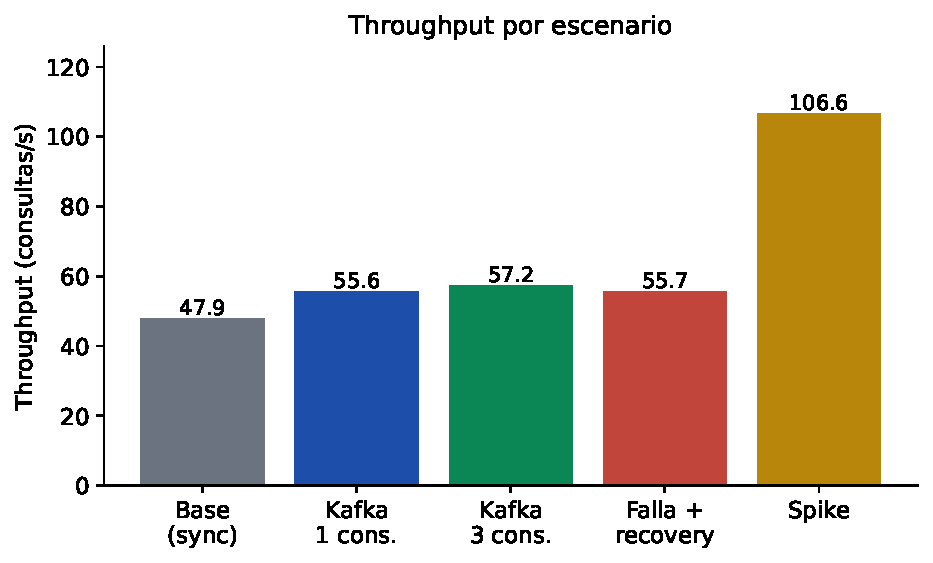
\includegraphics[width=0.72\textwidth]{figs/fig_t3_throughput}
\caption{Throughput procesado por escenario.}
\label{fig:throughput}
\end{figure}

\noindent
El modo asíncrono (\texttt{kafka\_1c}, 55,6 q/s) iguala o supera al
\texttt{base\_sync} (47,9 q/s) en \emph{throughput}, pero el cambio cualitativo
clave está en \emph{dónde vive la latencia}. En modo síncrono, el cliente sufre
una latencia de \emph{miss} de hasta \textbf{4,27\,s} en p95: 16 \emph{workers}
concurrentes golpean un Generador de Respuestas de un solo hilo con cómputo
\texttt{pandas} bloqueante, generando contención. En modo asíncrono, esa misma
operación vista por \texttt{cache\_service} cae a $\sim$0,27\,s (p95 de
\emph{miss}) porque los consumidores la \emph{serializan}; la espera no
desaparece, se traslada al \textbf{backlog de la cola} (Fig.~\ref{fig:latency}).
\textbf{Conclusión:} el desacoplamiento convierte la latencia de bloqueo del
cliente en \emph{backlog} elástico --- el productor nunca se bloquea, lo que
habilita la absorción de ráfagas y la tolerancia a fallos.

\subsection{Latencia extremo a extremo (E2E)}
\begin{figure}[H]
\centering
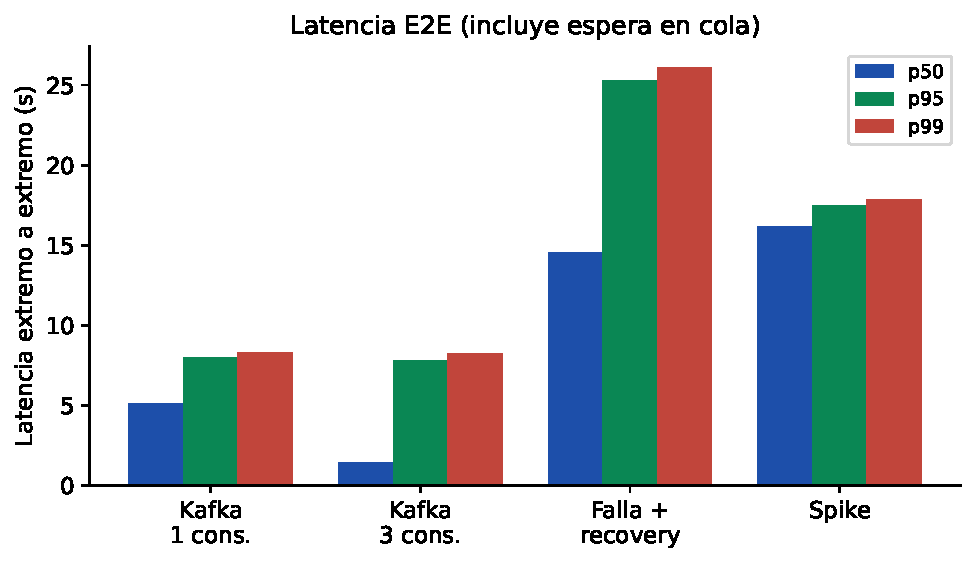
\includegraphics[width=0.78\textwidth]{figs/fig_t3_latency}
\caption{Latencia E2E (desde \texttt{created\_at} hasta el procesamiento). Incluye el tiempo de espera en cola.}
\label{fig:latency}
\end{figure}

\noindent
Las latencias E2E de varios segundos no indican un sistema lento, sino que el
ritmo de \emph{ingesta} (60--250 q/s) supera la capacidad del backend, por lo
que los mensajes esperan en cola. Es el comportamiento esperado y deseable: la
cola actúa como amortiguador. El caso \texttt{failure} exhibe la mayor p95
(25,3\,s) porque, durante la caída, los \emph{misses} se acumulan; el caso
\texttt{spike} mantiene una p95 menor (17,5\,s) pese al mayor volumen, porque
opera con 2 consumidores y nunca pierde el backend.

\subsection{Escalamiento de consumidores (DoD 3)}
\begin{figure}[H]
\centering
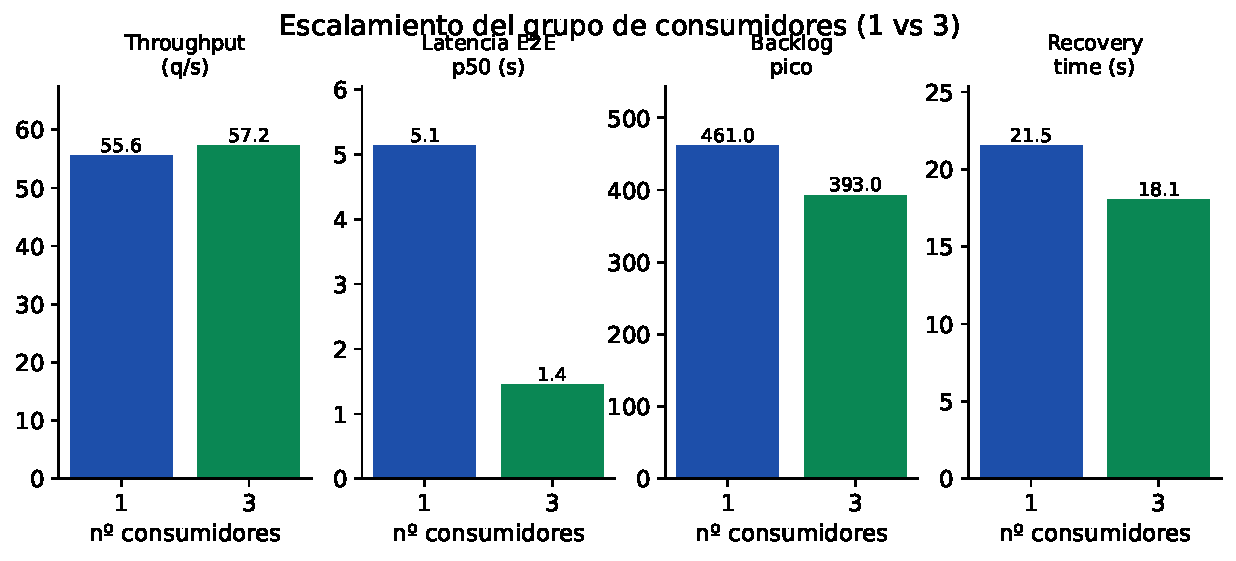
\includegraphics[width=0.95\textwidth]{figs/fig_t3_scaling}
\caption{Escalamiento de 1 a 3 consumidores: throughput, latencia E2E p50, backlog pico y recovery time.}
\label{fig:scaling}
\end{figure}

\noindent
Pasar de 1 a 3 consumidores casi no mueve el \emph{throughput} sostenido
($55{,}6\to57{,}2$ q/s). La razón es de manual de sistemas distribuidos: el
\textbf{cuello de botella es el Generador de Respuestas} (un solo \emph{worker}
con cómputo bloqueante de 30--120\,ms), no la capa de consumo. Sin embargo,
escalar \textbf{sí} mejora otras dimensiones: la latencia E2E mediana cae
\textbf{3,5$\times$} ($5{,}13\to1{,}45$\,s), el \emph{backlog} pico baja
($461\to393$) y el \emph{recovery time} mejora ($21{,}5\to18{,}1$\,s). Es decir,
más consumidores drenan los \emph{hits} (que no tocan el backend) en paralelo y
vacían la cola más rápido. \textbf{Lección:} escalar la capa de consumo ayuda
hasta el siguiente cuello de botella; para aumentar el \emph{throughput}
sostenido habría que escalar también el Generador de Respuestas.

\subsection{Tolerancia a fallos y recuperación (DoD 4)}
\begin{figure}[H]
\centering
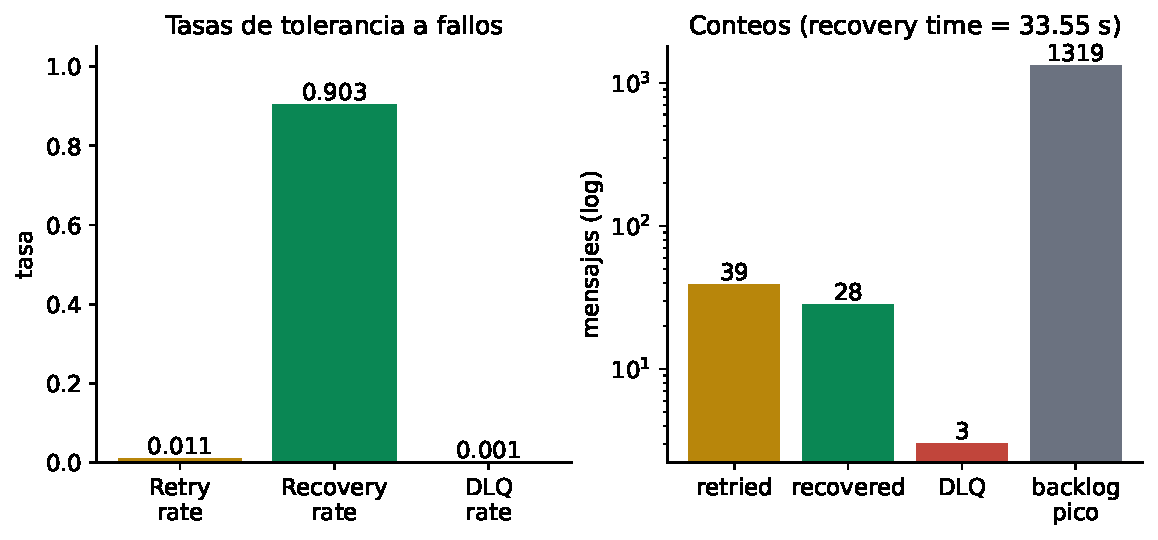
\includegraphics[width=0.95\textwidth]{figs/fig_t3_faults}
\caption{Escenario de falla: tasas y conteos de reintentos, recuperación y DLQ.}
\label{fig:faults}
\end{figure}

\noindent
Durante la caída simulada del Generador de Respuestas se dispararon
\textbf{39 reintentos}; de los mensajes que entraron al \emph{pipeline} de
reintentos, el \textbf{90,3\,\%} se recuperó ($recovery\ rate = 0{,}903$:
28 recuperados, solo 3 a la DLQ). El \emph{backlog} creció hasta
\textbf{1319} mensajes y se drenó por completo en \textbf{33,5\,s} tras
restaurar el backend (Fig.~\ref{fig:backlog}). Dos observaciones:
\begin{itemize}[noitemsep]
  \item La \emph{hit rate} se mantuvo alta (0,907) durante la falla: una caída
        del Generador de Respuestas no afecta a los \emph{hits} cacheados, que
        se siguen sirviendo. El sistema degrada parcialmente, no totalmente.
  \item El \emph{backoff} de reintentos es lo que produce el alto
        \emph{recovery rate}: los mensajes esperan a que el backend vuelva en
        lugar de agotarse hacia la DLQ. \textbf{Ninguna consulta se perdió en la
        red}; las 3 que llegaron a la DLQ quedan disponibles para inspección.
\end{itemize}

\subsection{Absorción del \emph{spike} (DoD 5)}
\begin{figure}[H]
\centering
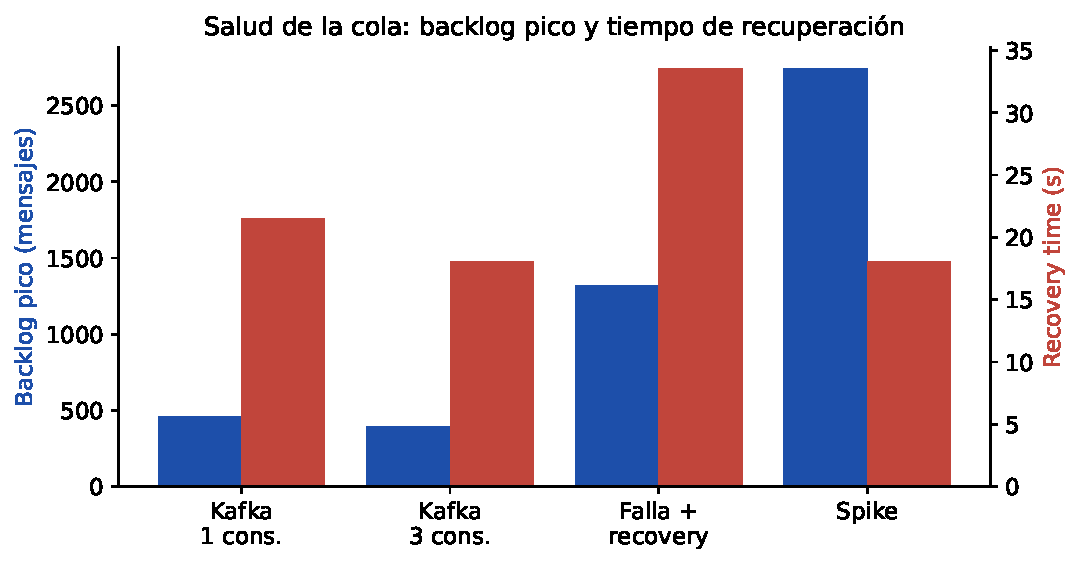
\includegraphics[width=0.78\textwidth]{figs/fig_t3_backlog}
\caption{Salud de la cola: backlog pico y recovery time por escenario.}
\label{fig:backlog}
\end{figure}

\noindent
Al conmutar la tasa de $40$ a $250$ q/s, el sistema \textbf{no colapsó}:
procesó 7564 mensajes (throughput promedio 106,6 q/s), el \emph{backlog} absorbió
el exceso (pico \textbf{2743}) y se drenó en \textbf{18,1\,s}, con
\textbf{0 errores y 0 mensajes en la DLQ}. Esto evidencia la propiedad central
de las arquitecturas dirigidas por eventos: la cola desacopla la tasa de
producción de la de consumo, suavizando ráfagas que en el modelo síncrono
habrían saturado al backend y propagado errores al cliente.

% ============================================================ %
\section{Discusión}
% ============================================================ %
\begin{itemize}
  \item \textbf{Síncrono vs.\ asíncrono.} El modo síncrono ofrece menor latencia
        por petición \emph{cuando hay holgura}, pero acopla cliente y backend:
        bajo carga, la latencia de \emph{miss} se dispara (4,27\,s p95). El modo
        asíncrono nunca bloquea al productor y transforma la sobrecarga en
        \emph{backlog} medible y recuperable.
  \item \textbf{Escalabilidad acotada por el backend.} El experimento confirma la
        teoría de colas: añadir consumidores reduce latencia y acelera la
        recuperación, pero el \emph{throughput} de estado estable está limitado
        por el servicio más lento de la cadena.
  \item \textbf{Tolerancia a fallos efectiva.} La combinación de reintentos con
        \emph{backoff} + DLQ logra recuperar el 90\,\% de los mensajes ante una
        caída transitoria, sin pérdidas, y aísla en la DLQ los casos
        irrecuperables.
\end{itemize}

\paragraph{Limitaciones.} El broker Kafka es de nodo único (\emph{replication
factor} 1), adecuado para la evaluación pero no tolerante a la caída del propio
broker. El \emph{recovery time} se mide a nivel de drenado de backlog (no por
mensaje individual). El Generador de Respuestas, al ser monohilo y bloqueante,
acota el \emph{throughput} global.

% ============================================================ %
\section{Conclusiones}
% ============================================================ %
La migración a una arquitectura asíncrona basada en Kafka cumple la totalidad de
las Épicas y de la Definición de Terminado. El sistema resultante: (i) desacopla
ingesta y procesamiento, absorbiendo un \emph{spike} de $40\to250$ q/s sin
pérdidas; (ii) escala horizontalmente el grupo de consumidores, mejorando la
latencia mediana $3{,}5\times$ y el \emph{recovery time}; y (iii) tolera caídas
del backend recuperando el 90\,\% de las consultas mediante reintentos con
\emph{backoff} y aislando el resto en una DLQ. Los KPIs de salud de cola
(\emph{backlog}, \emph{recovery time}) y de tolerancia a fallos
(\emph{retry/recovery/DLQ rate}) hacen observable el comportamiento asíncrono, y
confirman empíricamente las propiedades esperadas de un sistema distribuido
dirigido por eventos.

% ============================================================ %
\appendix
\section{Reproducción}
\begin{lstlisting}[caption={Comandos para reproducir la batería}]
# Levantar el stack
docker compose up -d --build

# Batería completa (5 escenarios del DoD)
python experiments/run_async.py --scenario all

# Figuras del informe
python experiments/build_figures_async.py

# Inspección del grupo / lag por tópico
docker compose exec kafka /opt/kafka/bin/kafka-consumer-groups.sh \
  --bootstrap-server localhost:9092 --describe --group cache-consumers
\end{lstlisting}

\section{Parámetros clave (\texttt{.env})}
\begin{lstlisting}
MAX_RETRIES=3        # fallas antes de expulsar a la DLQ
RETRY_DELAY_MS=1000  # backoff antes de re-encolar a reintentos
PARTITIONS_MAIN=6    # particiones del topico principal (>= replicas)
CACHE_POLICY=LRU     # cache congelada
REDIS_MAXMEMORY=200mb
\end{lstlisting}

\end{document}
